\documentclass{llncs}

\usepackage[pdftex]{graphicx}
\usepackage{amsmath}

\usepackage[T1]{fontenc}
\usepackage{indentfirst}
%\usepackage{natbib}
\usepackage{xcolor,graphicx,url}
\usepackage[utf8]{inputenc}
\usepackage{amsmath}
\usepackage{graphicx}
\usepackage{url}
\usepackage{algorithm}
\usepackage{algorithmic}
\usepackage{graphicx}
\usepackage{lipsum}


\begin{document}

\title{Improving the Generation of Earthquake Risk Models Using
  Evolutionary Algorithms Tempered by Domain Knowledge}

\author{
  Yuri Lavinas\inst{1} \and 
  Xiucai Ye\inst{2} \and 
  Marcelo Ladeira\inst{3} \and 
  Claus Aranha\inst{4}
}

\institute{ 
  University of Brasilia, Computer Science Department
  \email{yclavinas@gmail.com} \and 
  University of Tsukuba, Graduate School of SIE 
  \email{yexiucai@mma.cs.tsukuba.ac.jp} \and 
  University of Brasilia, Computer Science Department 
  \email{mladeira@unb.br} \and 
  University of Tsukuba, Graduate School of SIE
  \email{caranha@cs.tsukuba.ac.jp}}

\maketitle

\begin{abstract}
Earthquake Risk Models describe the risk of occurrence of seismic
events on a given area based on information such as past earthquakes
in nearby regions and the seismic properties of the area under study.
These models can be used to help to better understand earthquakes,
their patterns and their mechanisms.

In previous work, we showed that Genetic Algorithms (GA) could
generate risk models with the same degree of precision as the Relative
Intensity (RI) method, which is considered a benchmark for this
problem.  However, a few shortcomings were also defined in that
approach: (1) The representation of the model in the Genetic Algorithm
was too sparse, (2) Domain knowledge was not used to create the model,
and (3) The relationship between foreshocks and aftershocks were not 
taken into account.

In this work, we try to address these three concerns. We propose a new
representation of a seismic risk model to be used as the genome of the
Genetic Algorithm. We introduces a hybrid model that incorporates
seismic theories about earthquake distribution (such as the Omori-Utsu
formula). And we use clustering to filter the earthquake catalog in
order to remove earthquakes that are likely to be aftershocks before
generating the risk model.

We examine each of these changes through simulations using the catalog
of Japanese earthquakes between 2000 and 2010. According to our
results, clustering the earthquake catalog produces better models,
while the proposed changes to representation did not show such a clear
effect. These results allow us to draw recommendations for future
developments.

\end{abstract}

% Main file with the paper
%%%%%%%%%%%%%%%%%%%%%%%%%%%%%%%%%%%%%%%%%%%%%%%%%%%%%%%%%%%%%%%%%%
\section{Introduction}\label{intro}

% Why are we studying this problem
Earthquakes can cause great damage to human society through soil
rupture, movement, tsunami, etc. Some recent earthquakes that
highlight this destructive potential are the great East Japan
Earthquake of 2011 (Figure~\ref{GreatEastJapan}), and the
April 2015 earthquake in Nepal. One important tool for the enactment
of policies that minimise the consequences of these events are
earthquake occurrence models (also called risk models). These models
can be used to identify patterns in the seismic mechanisms that
generate earthquakes, and are important to increase our understanding
of these events.


% \cite{ecta14} opening image. Would be better to have a clustered one.
\begin{figure}[]
\centering
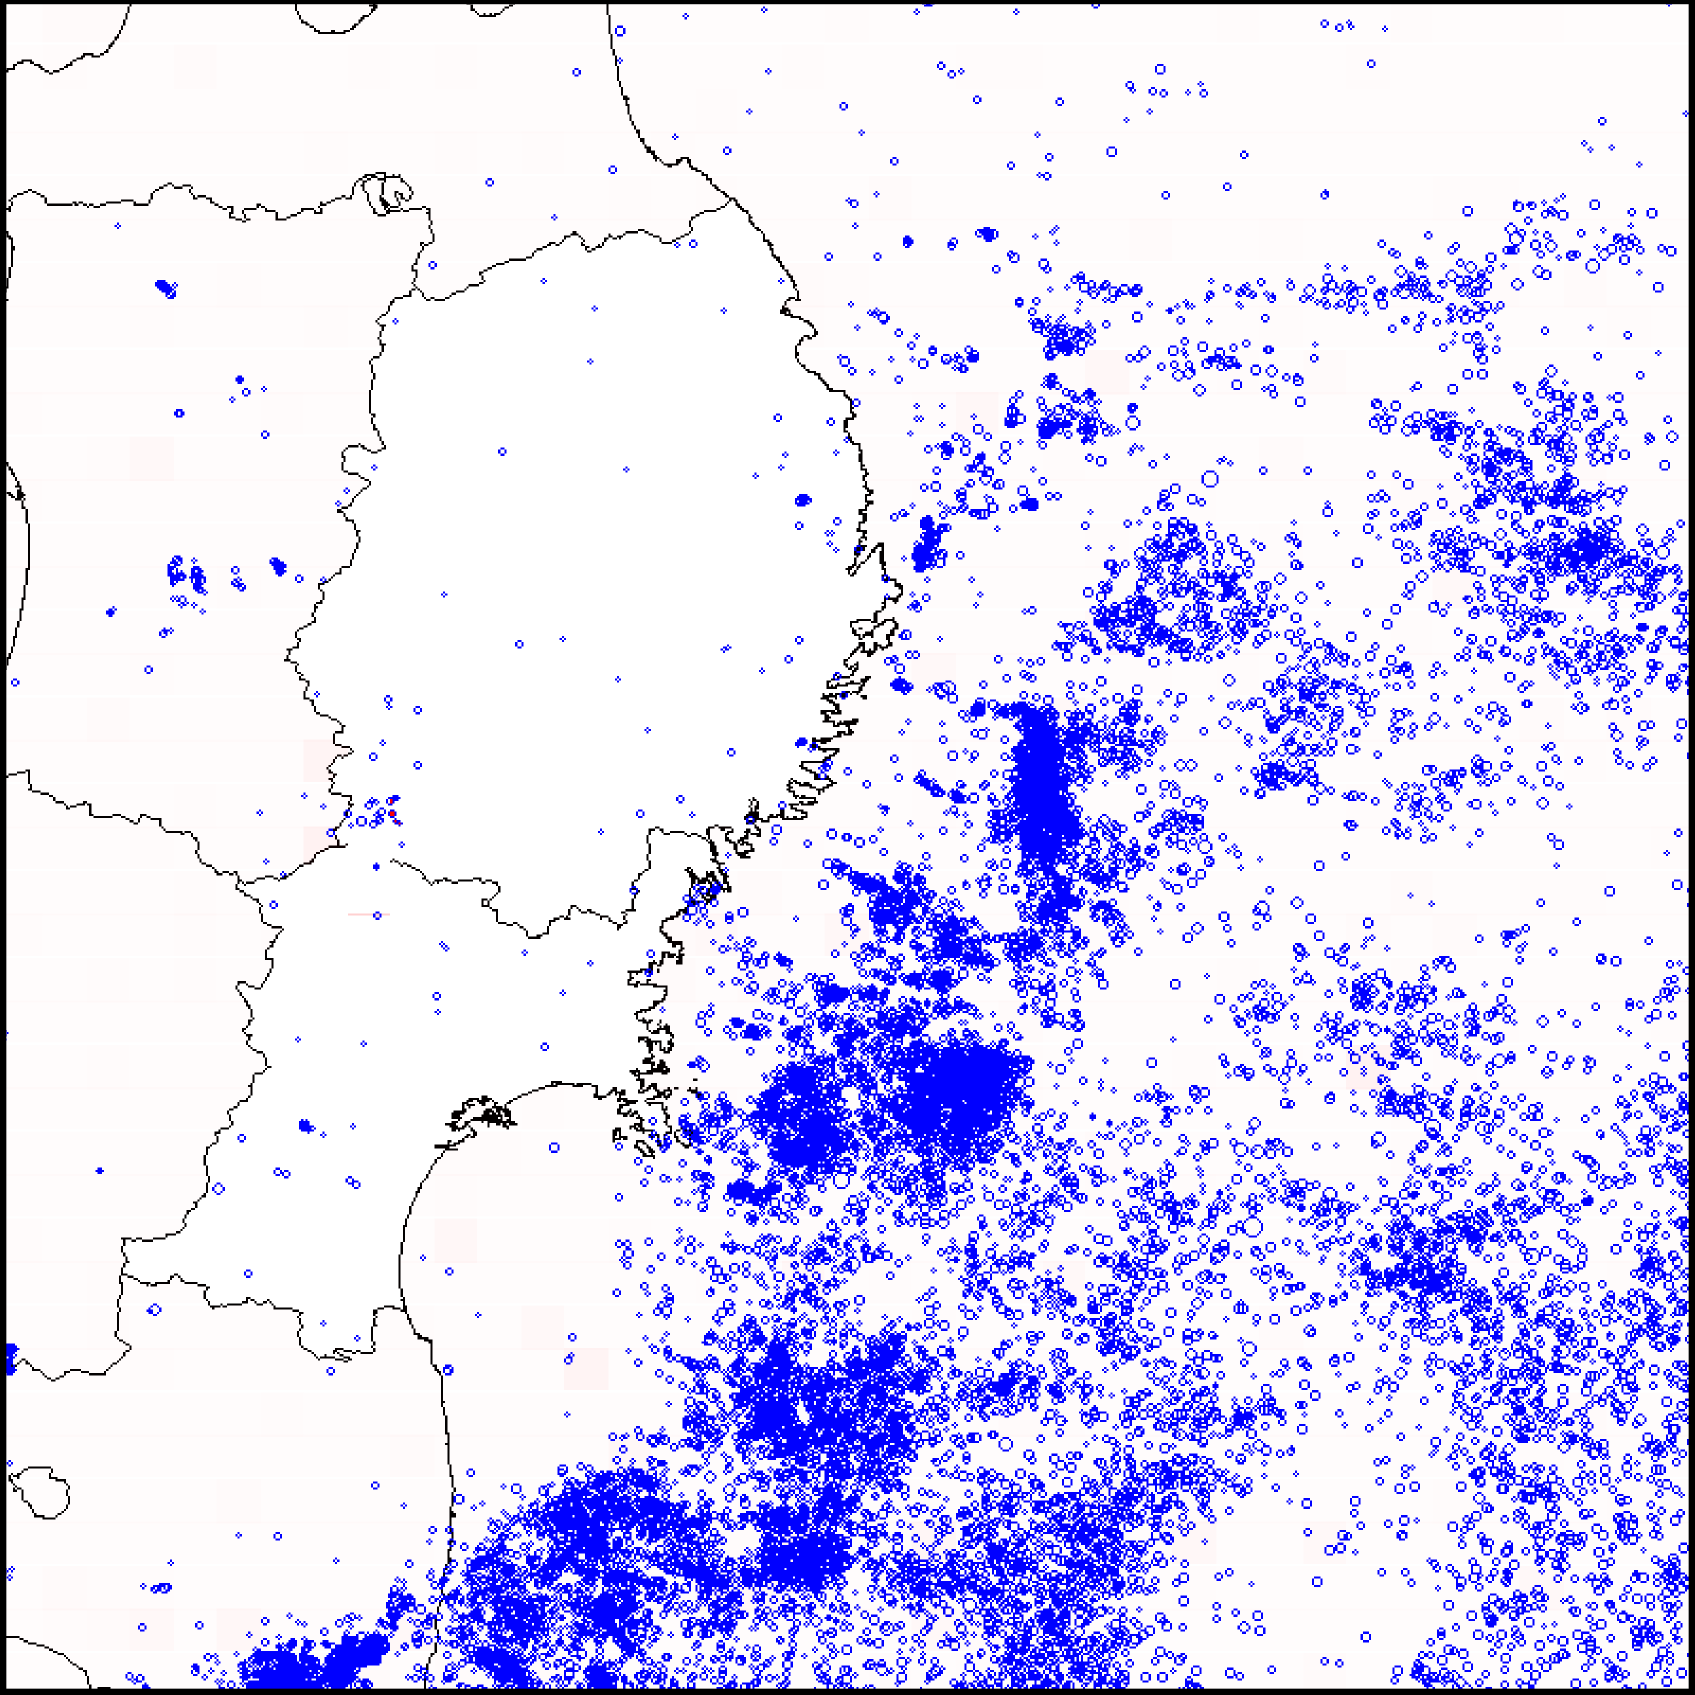
\includegraphics[width=.45\textwidth]{img/earthquakes2011.png}
\caption{Seismic Activity in Eastern Japan in 2011. Each dot
  shows one earthquake}
\label{GreatEastJapan}
\end{figure}

% Context of our work
In our previous work~\cite{ecta14}, we proposed a way to generate
earthquake risk models using a standard Genetic Algorithm (here called
the GAModel). The GA model was shown to be competitive with the
Relative Intensity (RI) model, while not using any a-priori
information about the distribution of earthquake occurrences. In this
paper, we identify three key issues with the GAModel, and propose
adjustments to the algorithms that address these issues.

The first issue is that the genome representation used by GAModel has
too many parameters (over 2000 for regular cases), leading to an
unnecessarily large search space. To address this issue, we propose a
new genome representation for an earthquake risk model, the
\emph{Reduced Representation}. In this representation only those
locations with a minimal probability of earthquake are represented as
parameters in the evolutionary process.

% Second issue: Hybridization with domain knowledge
The second issue is that GAModel does not take into account any sort
of domain knowledge, such as the assumption that earthquakes cluster
in both time and space. Heuristic search methods usually benefit from
the introduction of domain knowledge to the search. Therefore, we
propose a hybrid version of the GAModel which incorporates seismic
models of earthquake decay. In a two step process, the Genetic
Algorithm first generates a set of mainshocks, then uses an adaptation
of the Epidemic Type Aftershock Sequence
(ETAS)~\cite{zhuang2004analyzing} to generate the aftershocks.

The third issue is the examination of ``de-clustering'' effects in the
historical catalog used for generating the risk model. In seismology,
de-clustering refers to the act of identifying earthquakes as either
mainshocks or aftershocks, and removing all but the main shocks from
the catalog, which is considered the representative earthquake for the
group. Accordingly, a de-clustered earthquake catalog is considered to
be easier to study, given that the de-clustering process removes
redundant information~\cite{van2012seismicity}. In this work, we
generate the de-clustered catalog by grouping earthquakes in space and
time using Spectral Clustering~\cite{spectral_tutorial}.

These adaptions are described in detail in
section~\ref{sec:adaptations}. We compare the contributions of each
adaptation to the generation of models based on the earthquake catalog
of the Japanese archipelago, between 2000 and 2010. The set up of this
experiment is described in section~\ref{sec:experiment}, and the main
results are listed in section~\ref{sec:results}.  Our results indicate
that the clustering pre-processing step gives the biggest contribution
to the model precision, and that the new representation reduces the
search space without negatively affecting the model results.


\section{Background}
\label{sec:background}

An Earthquake Risk model states the probability of earthquake
occurrence on a defined area and time period. These models are often
based on past occurrence of earthquakes (historical catalogs).  They
can also make use of seismic properties of the area under study, such
as faults, terrain properties, etc.

The ``prediction'' of earthquakes is a polemic subject, and no
research so far has come close to suggesting that individual large
scale earthquakes can be predicted. On the other hand, there is value
on the study of earthquake mechanisms and the generation of
statistical models of earthquake risk~\cite{Nature1999}.

In our previous work~\cite{ecta14}, we use a Genetic Algorithm (GA) to
optimise an Earthquake Risk Model, which is described in the framework
proposed by the Collaboratory for the Study of Earthquake
Predictability (CSEP).

The CSEP framework defines a model in reference to a geographical
region and a time period~\cite{zechar2010evaluating}. The geographical
region is divided in a grid, where each cell in the grid is called a
bin.

The model defines a number of expected earthquakes for each bin.  This
number must be a positive integer. A good model is one where the
number of estimated earthquakes in each bin corresponds to the actual
number of earthquakes that occurs in that bin during the target time
interval.

%%%%%%%%%%%%%%%%%%%%%%%%%%%%%%%%%%%%%%%%&&&&&&&&&&&&&&&&&&&&&&
\subsection{The GAModel}\label{sec:background:gamodel}

Using the CSEP framework described in the previous subsection, we
proposed the GAModel~\cite{ecta14}, which uses Genetic Algorithms to
generate an earthquake risk model based on earthquake catalog data.

In the GAModel, each individual is treated as a prediction in the CSEP
framework. The fitness of each individual will be calculated using the
log-likelihood of the catalog data given the individual's prediction.

\subsubsection*{Genome Representation and Evolutionary Operators.}

Each individual is represented as real valued array, where each
element is a bin, with an associated number of earthquakes. One-point
crossover, elitism and polynomial bounded mutation are used as
evolutionary operators. The relevant parameters were set as Elite Size
= 1, Crossover chance = 0.9, Mutation Chance = 0.1, Polynomial Bounded
parameters eta = 1, low = 0, up = 1.


\subsubsection*{Fitness Function and Selection.}

Let an individual $\Lambda = \{\lambda_1, \lambda_2, \ldots,
\lambda_N\}$ be a forecast in the CSEP framework. Let the set of
earthquake occurrences from the catalog be $\Omega = \{\omega_1,
\omega_2, \ldots, \omega_N\}$. The log-likelihood of the catalog data
given an individual is calculated as:

\begin{equation}
L(\Omega|\Lambda) = \sum_{i=1}^{n}L(\omega_i|\lambda_i) \\ =
\sum_{i=1}^{n} -\lambda_i + \omega_i\log\lambda_i - \log\omega_i! .
\end{equation}

To avoid overfitting, the period under consideration is divided into
sub-periods, the log-likelihood for each sub-period is calculated
separately, and the worst value is used as the fitness~\cite{ecta14}.

\subsection{Related Literature}

The usage of Evolutionary Computation (EC) in the field of earthquake
risk models is somewhat sporadic. Zhang and Wang~\cite{Zhang2012} used
Genetic Algorithms to fine tune an Artificial Neural Network (ANN) and
used this system to produce a forecast model. Zhou and
Zu~\cite{Feiyan2014} also proposed a combination of ANN and EC, but
their system forecasts only the magnitude parameter of
earthquakes. Sadat, in~\cite{sadat2015application}, used ANN and GA to
predict the magnitude of the earthquakes in North Iran.

%Fault Model parameters
There are more works when we discuss EC methods and estimation of
parameter values in seismological models. Nicknam et
al.~\cite{Nicknam2010} simulated some components from a seismogram
station and predicted seismograms for other stations. They combined
the Empirical Green’s Function (EGF) with GA. Kennett and
Sambridge~\cite{Kennett1992} used GA and associated teleseisms
procedures to determine the Fault Model parameters of an
earthquake.

%PGA
Another popular approach is to use EC methods do calculate the Peak
Ground Acceleration (PGA) parameter. The works done by Kerh et
al.~\cite{Kerh2010, Kerh2015} are a combination of ANN and GA to
estimate or predict PGA in Taiwan. Cabalar and
Cevik~\cite{Cabalar2009} work also aimed to predict the PGA, but their
work uses genetic programming (GP) and use strong-ground-motion data
from Turkey.

%Jafarian et al.~\cite{jafarian2010empirical}, used GP to develop an
%empirical predictive equation $v_max/a_max$ ratio of the shallow
%crustal strong ground motions recorded at free field sites. They found
%a relation between the $v_max/a_max$ and the earthquake magnitude and
%the source-to-site distance.
 
Ramos and Vázques~\cite{Ramos2011} used Genetic Algorithms to decide
the location of sensing stations. In this work they achieved, in
general, better results with the GA method when compared with the
Seismic Alert System (SAS) method and a greedy algorithm
method.

%Saeidian et al.~\cite{saeidian2016evaluation} work also based
%on the same idea of locating sensing stations. They do a comparison in
%performance between the GA and Bees Algorithm (BA) to decide which of
%those techniques would perform better when choosing the location of
%sensing stations. He found out that the GA was faster than the BA.

%Huda and Santosa \cite{ijse5762} published a paper in which the goal
%was to find, via GA, the speed of the waves P and S in the mantle and
%in the earth crust. P waves are indicated as the first fault found in
%seismological data and S waves are the changes caused in the phase of
%a P wave~\cite{ijse5762}. This work aimed to obtain a structure of the
%Japanese underground.

% TODO: No SPACE!
 
\section{Proposed Changes}
\label{sec:adaptations}

In this work, we propose three improvements to the GAModel: A reduced
genome representation, Hybridisation with the ETAS empirical model,
and the clustering of the earthquake catalog. Each of these changes
are described below.

%%%%%%%%%%%%%%%%%%%%%%%%%%%%%%%%%%%%%%%%%%%%%%%%%%55
\subsection{Reduced Genome Representation}

In the GAModel, problem is represented as a vector $X$ where each bin
corresponds to an element in the vector. As the number of bins in a
region numbers into the thousands, this representation leads to a huge
search space to be explored.

We have observed that in many cases, the vector of catalog
earthquakes is sparse. In other words, most of the elements of $X$
will be zero or close to it. To use this fact to decrease the
search space, we propose a ``reduced'' representation of a risk Model.

A summary of the reduced representation is as follows: First, before
initialising the Genetic Algorithm, we estimate the expected total
number of earthquakes in the model based on the past data. Then, this
value is used as the total number of earthquakes to be added to the
model. The reduced representation will be a vector of bin coordinates
for each of these earthquakes, representing their position inside the
target area. This is much smaller than a representation including each
bin as an element.


\subsubsection*{Implementation}

The reduced representation is a vector $V$ of ordered pairs. The first
element of this pair is the integer index that identify a bin in the
model. The second element of the pair is the number of earthquake
occurrences estimated for this bin.

The size of the vector $V$ is calculated as the number of bins in the
historical catalog that contain at least one earthquake. For each
element in $V$, the bin index and the estimated number of occurrences
are drawn randomly from a uniform distribution.

To generate a model from the reduced representation, we need to go two
intermediate steps. The first one is to transform the reduced
representation into a regular representation. This is achieved by
copying the estimated value of an element to the bin indicated by
stored index for that element. Bins that are not indicated by any
element in the vector are set to zero estimated earthquakes.

The second step is to apply the inverse Poisson on the estimated
values to retrieve the number of earthquakes, as described in
algorithm~\ref{inversePoisson}.

\subsubsection*{Operators}

The reduced representation can use the same one point crossover as the
GAModel, but a different mutation operation is required. The mutation
operator works by selecting one element in the vector $V$, and drawing
new values for the index and the estimation parameter from a uniform
distribution.


%%%%%%%%%%%%%%%%%%%%%%%%%%%%%%%%%%%%%%%%%%%%%%%%%%%%%%%%%%%%%
\subsection{Hybridisation with ETAS}

% Motivation
The GAModel produces risk models without using any sort of domain
knowledge, other than the difference between the individual being
evaluated and the earthquake catalog data.

However, one simple observation that could be added to the GAModel is
that earthquakes cluster in space and time. Large earthquakes are
usually followed by a wave of smaller earthquakes, these pairings
being commonly known as \emph{mainshocks} and
\emph{aftershocks}~\cite{schorlemmer2010first}.

To include this idea into the GAModel, we modify the process which
generates a Model from an individual. In this modified process, one
individual will only produce mainshocks into the model, afterwards the
aftershock are derived from the mainshocks, using empirical seismic laws
such as the \emph{modified Omori Law}.

We define this hybridisation between empirical seismic laws and the
GAModel as the \emph{EMP-GA}. Below, we detail the implementation of
both steps.

%%%%%%%%%%%%%%%%%%%%%%%%%%%%%%%%%%%%%%%%%%%%%%%%%%%%%%%%%%%%%%%%%
\subsubsection*{Implementation}

The EMP-GA generates models with mainshocks and aftershocks following
a two-step procedure.

In the first step, we use the GAModel to generate a set of mainshock
earthquakes, which we will refer to as \emph{synthetic mainshock
  data}. In the second step, we use seismic empirical equations to
obtain the aftershocks from the synthetic mainshock data, and add them
to the model.

The process we use to generate aftershocks from the synthetic
mainshock data is inspired by the space-time epidemic-type aftershock
sequence (ETAS). The total number of earthquakes in a bin is given as
% TODO: Sentar com o Yuri e pedir para ele me explicar a
% implementacao/razao desta equacao detalhe por detalhe.
\begin{equation}\label{emp-model}
 \Lambda(t,x,y|\Upsilon_t) = [\mu(x,y) + \displaystyle\sum_{t_i \in t}
   K(M_i)g(t-t_i)P(x,y)]J(M).
\end{equation}
In this equation, $t$ is the target time for the model, $x,y$ are
latitude/longitude coordinates within the target area, $\Upsilon_t$ is
the number of mainshocks derived in the first step, $\mu(x,y)$ is the
expected number of earthquakes at the $(x,y)$ bin, $t_i$ is a time
interval within $t$, $K(M_i)$ is the total amount of triggered events,
$g(\Delta t)$ is the probability density form of the modified Omori
law, $P(x,y)$ is a function that distributes aftershocks in space
nearby the mainshock, and $J(M)$ is the ETAS simulated magnitude. Let
us explain each of these components below.

\subsubsection*{Omori's Law and Triggered Events}

The Omori law, which is considered to be an empirical seismic formula
which has withstood the test of
time~\cite{utsu1995centenary,omori1895after}, is a power law that
relates the magnitude of an earthquake with the decay of aftershock
activity over time. It can estimate the number of aftershocks based on
the mainshocks in the synthetic data generated by one individual in
the EMPGA. For this approach, we use the probability density function
(PDF) form of the modified Omori law~\cite{zhuang2004analyzing},
defined as

\begin{equation}\label{omori}
  g(\Delta t)= \frac{(p-1)}{c(1+ \frac{t}{c})^{-p}}.
\end{equation}

In this equation, $p$ and $c$ are
constants. Utsu~\cite{utsu1995centenary}, summarise the studies of
this formula for the Japan case, and describe a range for these
variables using the Davidon-Fletcher-Powell optimisation
procedure. These ranges, used in ETAS, are 0.9 to 1.4 for $p$, and
0.003 and 0.3 for $c$.

Also, $\Delta t$ is the time interval for how long a mainshock may
influence or cause an aftershock. According to
Yamanaka~\cite{yamanaka1990scaling}, this value must be chosen
carefully, for a value too short will lead to a small number of
aftershocks, while a value too long might confound aftershocks and
background activity. His work suggests the values $p = 1.3$, $c =
0.003$, and $\Delta t = 30$ days, which we use in this paper.

The total amount of events triggered by a mainshock is represented in
equation~\ref{emp-model} as $K(M_i)$. To calculate this value,
we count the number of aftershocks within a given area $A$ from
the mainshock, using the formula

\begin{equation}\label{triggered}
 K(M_i) = A\ exp([\alpha(M_i-M_c)]).
\end{equation}

Where $M_c = 3.0$ is the magnitude threshold and $\alpha(M)$ is defined
as the inverse of the magnitude, according to
Ogata~\cite{ogata2006space}. The area $A$ is obtained using the
equation from Yamanaka~\cite{yamanaka1990scaling}

\begin{equation}
A = e^{(1.02M -4)}.
\end{equation}

Using the number of triggered events per magnitude $K(Mi)$, and the
Modified Omori PDF $g(t)$, it is possible to calculate the total
number of earthquakes generated from a mainshock, by iterating
over $t_i$:
\begin{equation}
\displaystyle\sum_{t_i \in t} K(M_i)g(t-t_i)
\end{equation}

% TODO: From this description, it does not seem that P(x,y) is actually
% part of equation emp-model: double check with Yuri.
The resulting aftershocks need to be spread on bins near the mainshock
position. The $P(x,y)$ component of equation~\ref{emp-model} fills
this role. It calculates the position of the aftershocks based on the
position of the original mainshock. It simply places each aftershock
either north, south, east or west of the mainshock, getting further
from the origin after each iteration, until there are no more events
to be placed.

%% This equation is not clear -- where is the component that place
%% Aftershocks further away from the origin?
%\begin{subequations}
%\begin{gather*}
%        model[x+y] = (aftershocks-[model[x]-2*x])/4;\\
%        model[x-y] = (aftershocks-[model[x]-2*x])/4;\\
%        model[x-y*row] = (aftershocks-[model[x]-2*x])/4;\\
%        model[x+y*row] = (aftershocks-[model[x]-2*x])/4
%\end{gather*}
%\end{subequations}

% TODO: but WHAT is J(M)?
Finally, $J(M)$ is obtained by using the function \emph{etasim}, from
the SAPP \textit{R} package~\cite{webSapp} that simulates magnitude by
Gutenberg-Richter’s Law.

The above equations are put together in algorithm~\ref{algoEquations}.

\begin{algorithm}[H]\label{algoEquations}
  \caption{Aftershock distribution from empirical laws}
  \begin{algorithmic}
    \STATE FOR EACH BIN:
    \IF {Number of earthquakes in bin > 12} % Why?
    \STATE {Reduce number of earthquakes in bin to 12}
    \ENDIF
    \STATE aftershocks = 0
    \STATE magnitude values for earthquakes in bin = J(M)
    % What does this mean?
    % \STATE model  = attributeMagnitudeToEarthquake(model, J(M) )
    % \STATE magnitudes = getMagnitudeMainshock(model)
    
    \FOR{magnitude in magnitudes} 
    \FOR{t in time} 
    \STATE aftershocks += g(t)*K(magnitude)
    \ENDFOR
    \ENDFOR
    % Need a more detailed algorithm for P(x,y)
    \STATE Use P(x,y) to distribute aftershocks to neighbour bins
  \end{algorithmic}
\end{algorithm}

% TODO: Probably needs a longer explanation of ETAS in the
% Bibliography section.

%%%%%%%%%%%%%%%%%%%%%%%%%%%%%%%%%%%%%%%%%%%%%%%%%%%%%%%%%%%%%%%%%5
\subsection{Clustering the Catalog Data}

The third adaptation to the GAModel that we study in this paper is the
clustering of the earthquake catalog data using Spectral
Clustering. Unlike the two adaptations described beforehand, this one
does not require any change on the algorithm itself, happening instead
as a data pre-processing step when building the model. After the
catalog data is pre-processed, the Genetic Algorithm is applied
normally, using the de-clustered data for fitness evaluation.

This pre-processing step aims to remove redundant information from the
catalog, by clustering together earthquakes which are closely related
in a mainshock/aftershock relationship~\cite{van2012seismicity}.

However, because it is difficult to determine exactly when two
earthquakes should be clustered together, we choose a non-supervised
method, Spectral Clustering, to generate the clusters.

Spectral Clustering involves constructing a similarity matrix of the
elements to be clustered, finding the k-Nearest-Neighbours graph (KNN)
based on the similarity matrix, calculating the Laplacian matrix of
the KNN graph, and performing k-means clustering on the eigenvectors
of this matrix.

One of the main characteristics of Spectral Clustering that make it
interesting for this problem is that it can be very computationally
efficient~\cite{Ye2016}. This is very important for the clustering of
earthquake data, since each data set can contain tens of thousands of
earthquakes.

\subsubsection*{Spectral Clustering Implementation}

Let the earthquake catalog data be represented as a vector $X = \{x_1,
x_2, \ldots, x_n\ in \Re_d\}$, where $n$ is the number of earthquakes
in the catalog, $d$ is the number of attributes that characterise an
earthquake in the catalog, and $K$ is the desired number of
clusters. The clusters are calculated following
algorithm~\ref{spectralclustering}

% TODO: Probably needs to include how to calculate KNN
\begin{algorithm}[H]\label{spectralclustering}
  \caption{Spectral Clustering}
  \begin{algorithmic}
    \STATE{Construct the similarity matrix S}
    \FOR{i in $X$}
    \FOR{j in $X$}
    \IF{$i$ and $j$ are connected in the KNN graph}
    \STATE{$s_{i,j} = \exp(-||x_i-x_j||^2/2\sigma^2$}
    \ELSE
    \STATE{$s_{i,j} = 0$}
    \ENDIF
    \ENDFOR
    \ENDFOR
    \STATE Matrix $D = n x n$ diagonal matrix where $d_{i,i} = \sum^n_{j=1}s_{ij}$
    \STATE Compute Matrix $L = D - S$
    \STATE Compute $K$ smallest eigenvectors of $L$
    \STATE Compute matrix $V = (v_{ij})_{nxK}$, using these eigenvactors as columns.
    \STATE Compute matrix $U = (u_{ij})_{nxK}$, normalising the rows
    of $V$ such as $u_{i,j} = v_{i,j}/\sqrt{\sum_jv^2_{ij}}$
    \STATE Let each row in $U$ represent a data point, and cluster
    these points using k-means
    \FOR{each point $x_i$ in $X$}
    \STATE Assign the cluster of $u_i$ to $x_i$
    \ENDFOR
  \end{algorithmic}
\end{algorithm}

In this algorithm, $||x_i-x_j||$ is the Euclidean distance between
data points $x_i,x_j$. We use the number of nearest neighbours equal to
five, and $\sigma$, the kernel parameter, equal to $100$.

% TODO: Minutes is divided by 1000 to make the values smaller
We cluster the earthquakes based on their latitude, longitude, time
(in minutes), and depth. By observing the distributions of the
eigenvectors, we defined the weight of each dimension in the algorithm:

\begin{itemize}
\item latitude and longitude: 150
\item time: 7
\item Depth: 0.5
\end{itemize}


% TODO: Change the tone of the introduction, talk about exploring the
% TODO: proposed changes

% TODO: Do not add captions in images (as opposed to axis
% TODO: names). Captions are better added in the latex instead.

\section{Experiment Design}
\label{sec:experiment}

In this paper we propose three improvements for the GAModel algorithm
that generates earthquake risk models using GA: A reduced
representation that limits the search space of the algorithm, a hybrid
model generation that uses domain knowledge, and the pre-processing of
the data using Spectral Clustering.

We are interested in determine what effect these improvements have on
the generation of earthquake risk models. To achieve this, we execute
a series of simulation experiments. In these experiments, we generate
earthquake models for each combination of the above modifications,
using historical earthquake catalog data from the Japanese
archipelago.

\subsection{Experiment Design}

% Comparison on only Kanto e East Japan
% Unless Yuri sends me the missing data.

% CHANGE HERE TO ADD FOUR REGIONS
Our experiment has a factorial design with three factors: Using the
reduced representation, Using the hybrid model, and clustering the
data set. For each combinations of these factors, we generate 10 models
for two target regions and 6 five-year periods, for a total of 120
models per combination.

% NOT SURE IF WE KEEP THE PER-AREA ANALYSIS OR NOT
We use ANOVA to test whether any of the combinations shows a
significant deviation in terms of model accuracy, represented as the
log-likelihood between the model and the catalog data. If this is
indicated, we compare each combination with the original algorithm
using Tukey HSD. We repeat this procedure for each of the two areas
separately as well. In each of these tests, we set $\alpha = 0.05$.

%%%%%%%%%%%%%%%%%%%%%%%%%%%%%%%%%%%%%%%%%%%%%%%%%%%%%%%%%%%%%%%%%%%%%%%5
\subsection{Data Sets}

%%% Four Regions (Kansai, Touhoku, EastJapan, Kanto)
%%% TWO Regions: EastJapan and Kanto
%%% Six time periods (2005,2006,2007,2008,2009,2010)
%%% Depth cut-offs: 100
%%% Magnitude cutoff: 3

We use the earthquake catalog made available by the \emph{Japan
  Meteorological Agency} (JMA) webpage. From this catalog, we use the
following earthquake data: time of occurrence, magnitude, latitude,
longitude and epicentre depth.

% Areas we define
From this catalog, we focus on two areas for our study.

\emph{Kanto} is the region around metropolitan Tokyo. In this work we
define it as the area within latitude 34.8N to 37N and longitude
138.8W to 141W. It is divided into 2025 bins of approximately
25km$^2$.

\emph{East Japan} region covers the east coast of Japan, including a
large ocean area. In this work we define it as the area within
latitude 37N to 41N, and 140W to 144W. It is divided into 1600 bins of
approximately 100km$^2$.

% Kanto -> not in the oceanic plaque
% East Japan -> oceanic plaque

%\textbf{Kansai} Kansai is the region that includes Kyoto, Osaka and
%many others historical cities. In this area, rather than Kanto area,
%there is a small seismic activity. Its coordinates are 34 North,
%134.5 West, with 1600 bins. Each bin covers an area of approximately
%25km$^2$.

%\textbf{Touhoku} Touhoku is the region in the North of the main
%Japanese island. It has some clusters of seismic activities during
%the years we studied. Its coordinates are 37.8 North, 139.8 West,
%with 800 bins. Each bin covers an area of approximately 100km$^2$.

% Time filtering and time slice
We use earthquakes from the JMA catalog that happen between 2000 and
2010~\footnote{We deliberately avoid using the 2011 catalog, as the
  occurrence of the Great East Japan earthquake caused an anomalous
  number of aftershocks, more than the past five years added
  together. We are interested in adding this event to our analyses in
  the future}. This is divided in 11 five-year overlapping periods
(2000--2005, 2001--2006, and so on), which are identified by the last
year in the period.

% Depth and Magnitude Filtering
For each period, we filter earthquakes from the catalog using the
following rules: 
\begin{itemize}
\item Depth of the earthquake must be under below 100km, as shallow
  earthquakes are considered to be more independent and easier to
  analyse~\cite{yamanaka1990scaling}.
\item Magnitude of the earthquake must be above 3. While the catalog
  lists some earthquakes with magnitude under 3, often such
  earthquakes escape detection, and thus introduce incompleteness to
  the catalog.
\end{itemize}


\section{Results}
\label{sec:results}

Table~\ref{tab:loglikelihood} summarizes the results of the
experiments comparing the eight combinations over the different
scenarios. The empirical hybridization is denoted as \emph{EMP}, and
the reduced representation as \emph{Red}.

\begin{table}
  \caption{Log Likelihood Values for each scenario and
    combination. Higher values correspond to better models. Values in
    bold are the two highest log likelihood for a scenario. Each value
    is the average of 10 runs.}
  \label{tab:loglikelihood}
  \begin{tabular}{|c|c|c|c|c|c|c|c|c|}
    \hline
    & \multicolumn{4}{|c|}{No Pre-processing} & \multicolumn{4}{|c|}{Spectral Clustering}\\
    Scenario & GA & Red & EMP & EMP-Red & GA & Red & EMP & EMP-Red\\
    \hline
    Kanto 2005 & -2291.4 & -2354.1 & -2345.1 & -2557.8 & {\bf-2202.7} & -2233.3 & {\bf-2203.7} & -2355.0\\
    Kanto 2006 & -2269.2 & -2317.3 & -2350.7 & -2520.0 & {\bf-2173.3} & -2203.1 & {\bf-2175.8} & -2313.5\\
    Kanto 2007 & -2204.9 & -2235.7 & -2293.3 & -2449.5 & {\bf-2104.1} & -2125.0 & {\bf-2110.3} & -2213.9\\
    Kanto 2008 & -2203.0 & -2273.2 & -2277.7 & -2501.0 & {\bf-2097.9} & -2124.3 & {\bf-2010.3} & -2245.7\\
    Kanto 2009 & -2375.6 & -2418.5 & -2463.6 & -2630.7 & {\bf-2279.1} & -2299.1 & {\bf-2282.4} & -2382.0\\
    Kanto 2010 & -2203.6 & -2296.6 & -2294.9 & -2534.4 & {\bf-2099.5} & -2125.0 & {\bf-2104.0} & -2249.8\\
    \hline
    EastJapan 2005 &-2442.8&-2394.9&-2633.6&-2588.4& {\bf-2099.6} & {\bf-2150.2} & -2177.4 & -2300.6 \\
    EastJapan 2006 &-2211.1&-2191.7&-2408.9&-2390.9&{\bf-1896.7}&{\bf-1960.4}&-1965.7&-2131.8\\
    EastJapan 2007 &-2112.2&-2100.5&-2305.1&-2294.9&{\bf-1821.9}&{\bf-1889.4}&-1914.4&-2070.0\\
    EastJapan 2008 &-4139.7&-4288.6&-4301.3&-4424.8&{\bf-3942.5}&{\bf-3989.1}&-4034.9&-4156.8\\
    EastJapan 2009 &-2281.2&-2221.2&-2498.9&-2416.5&{\bf-1948.5}&{\bf-1087.4}&-2043.7&-2164.5\\
    EastJapan 2010 &-2577.7&-2579.1&-2783.9&-2783.9&{\bf-2232.7}&{\bf-2291.3}&-2296.9&-2455.2\\
    \hline
  \end{tabular}
\end{table}

%% ANOVA ANALYSIS

To better understand these results, we perform an ANOVA analysis...

* Anova in all areas

Because the anova indicated a significant difference, we use Tukey's
HSD to see which combination showed this difference ...

* HSD Tukey against GAModel

%% HEAT MAP

To get a better intuition about what these results mean in concrete
terms, we show a selection of the actual models... (explain heat map)

\begin{figure}
\centering
\begin{subfigure}{.5\textwidth}
  \centering
  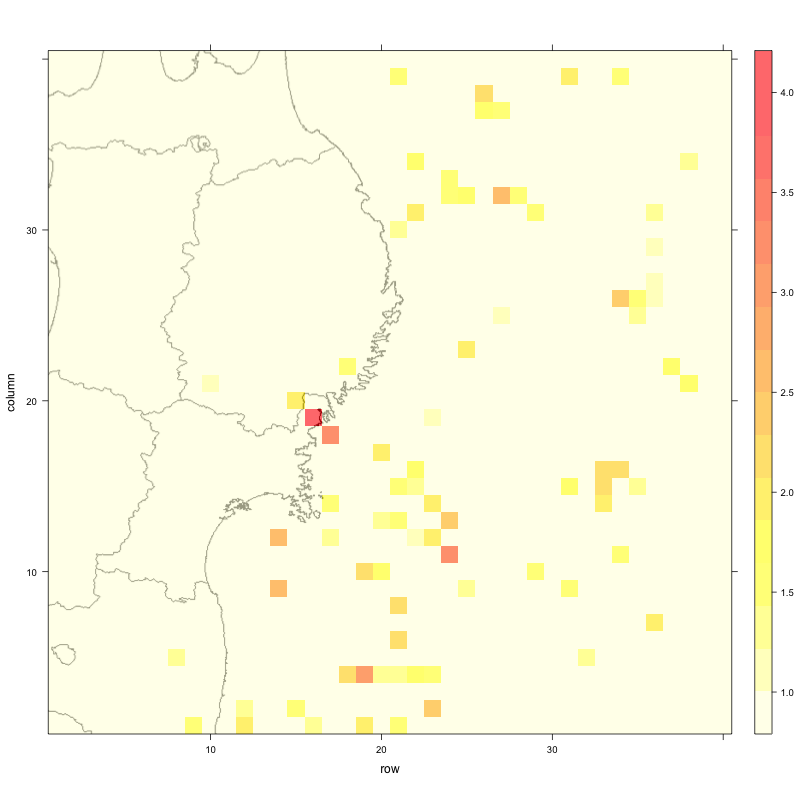
\includegraphics[width=1\linewidth]{img/gaModel}
  \caption{GAModel}
  \label{fig:sub1}
\end{subfigure}%
\begin{subfigure}{.5\textwidth}
  \centering
  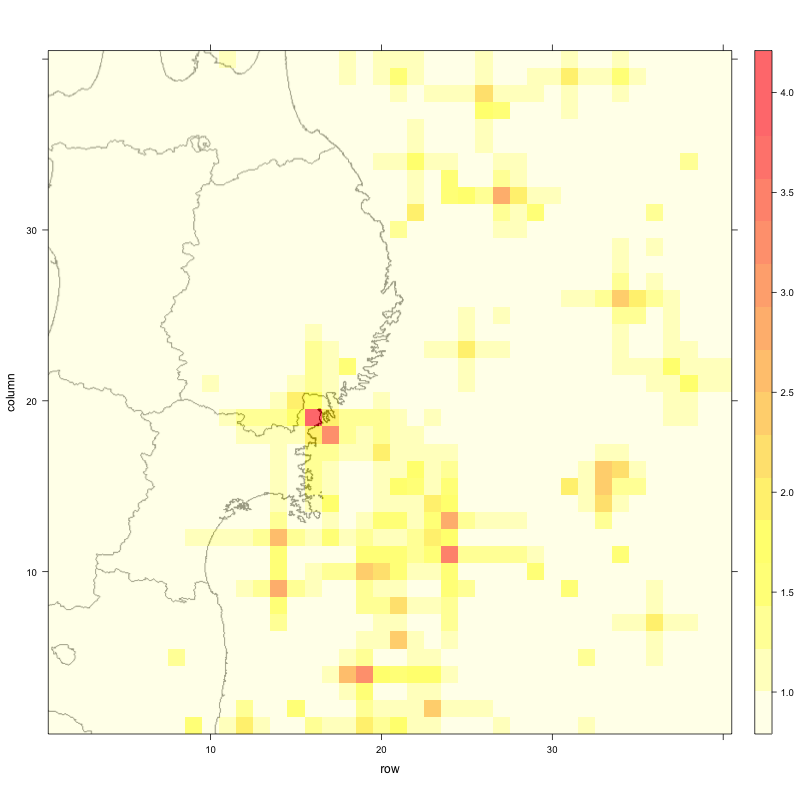
\includegraphics[width=1\linewidth]{img/SC-EMP-ga}
  \caption{Spectral Clustering with Emp-GA}
  \label{fig:sub2}
\end{subfigure}\\
\begin{subfigure}{.5\textwidth}
  \centering
  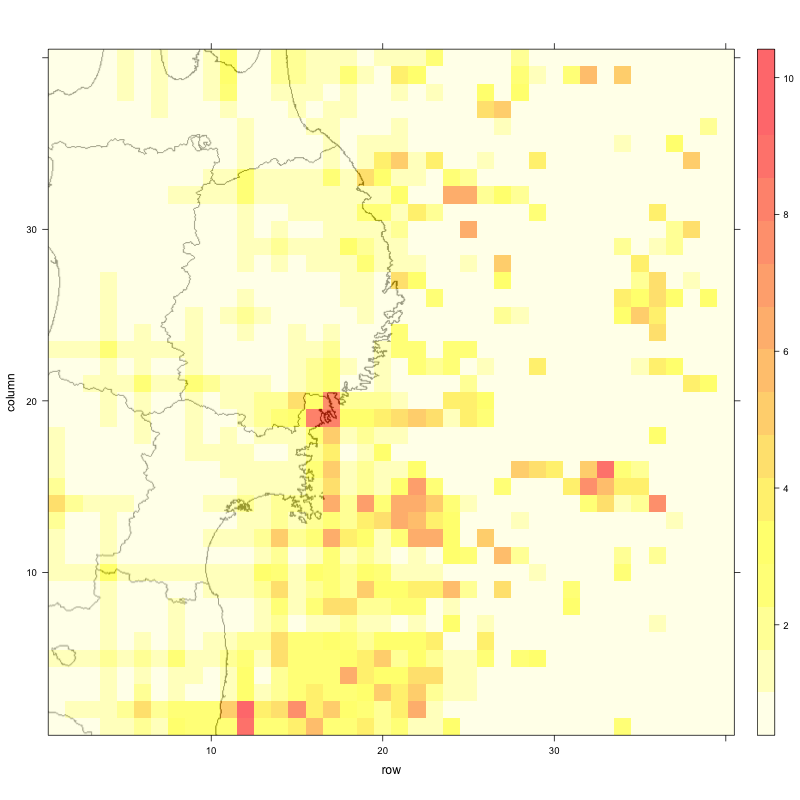
\includegraphics[width=1\linewidth]{img/EMP-RED-ga}
  \caption{EMP-GA with Reduced Representation}
  \label{fig:sub3}
\end{subfigure}%
\begin{subfigure}{.5\textwidth}
  \centering
  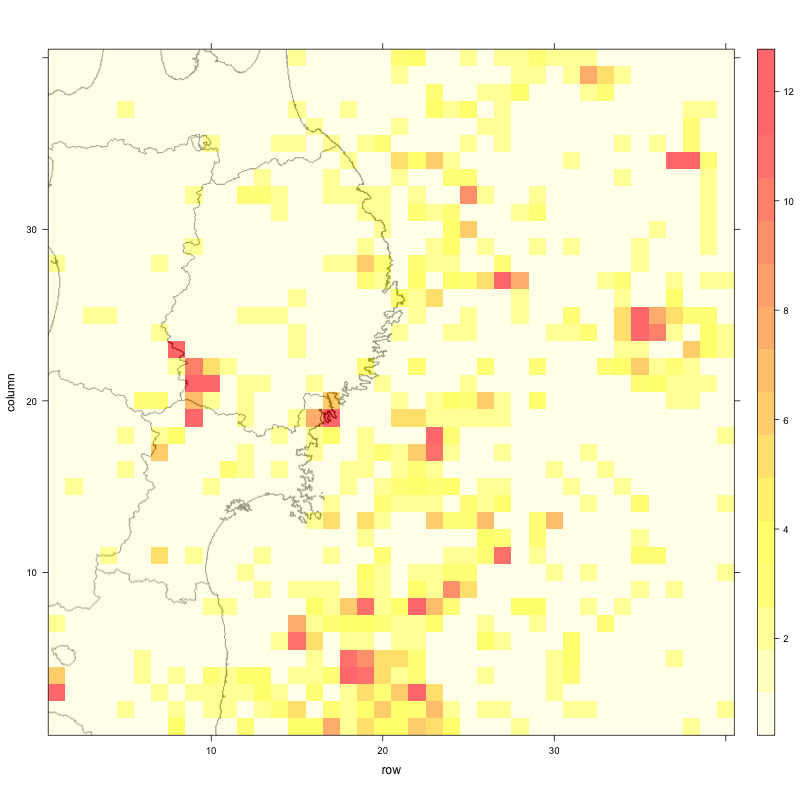
\includegraphics[width=1\linewidth]{img/realEastJapan_2010}
  \caption{Earthquake Catalog}
  \label{fig:sub4}
\end{subfigure}
\caption{Earthquake Risk Model Heatmaps, for scenario East Japan
  2010. Darker colors correspond to higher number of earthquakes}
\label{fig:test}
\end{figure}


\section{Discussion}
\label{sec:discussion}

Clustering is good. It is okay if Reduced GA is not worse, because
"lower search space"

\section{Conclusion}
\label{sec:conclusion}

(TO WRITE) We did many choices of the target regions and datas that made the
models easier to analyse. In future work, we would like to see the
results of removing these constraints from the data set, and how to
deal with this harder problem.


\subsubsection*{Acknowledgments.} 
The authors would like to thank the Japan Meteorological Agency for
making available the earthquake catalog used in this study.

\bibliographystyle{splncs03}
\bibliography{bib}

\end{document}
